\documentclass[a4paper,11pt,twoside,openright]{report}

\usepackage{graphicx}
\usepackage{ngerman}
\usepackage[utf8x]{inputenc}
\usepackage{fancyvrb}
\usepackage{courier}
\usepackage{helvet}
\usepackage{tikz}
\usepackage{xcolor}
\usepackage{pdfpages}
\usepackage[strict]{changepage}
\usepackage{subcaption}
\usepackage{enumitem}


\usepackage[english]{babel}
 
\usepackage{amsthm}
\usepackage{amssymb}
 
\theoremstyle{definition}
\newtheorem{definition}{Definition}[section]
 
\theoremstyle{remark}
\newtheorem*{remark}{Remark}

\pdfoptionpdfminorversion=6

% \definecolor{se_dark_blue}{RGB}{0,103,166} % powerpoint
\definecolor{se_dark_blue}{RGB}{0,96,178} % website
% \definecolor{se_light_blue}{RGB}{119,158,201} % powerpoint
\definecolor{se_light_blue}{RGB}{129,160,225} % website


%% setup listings
\usepackage{listings}
\lstset{
    numbers=left,
    numberstyle=\tiny,
    numbersep=5pt,
    xleftmargin=11pt,
    xrightmargin=4pt,
    frame=single,
    aboveskip=0pt,
    belowskip=-6pt,
    sensitive=true,
    float=!t,
    breaklines=false,
    captionpos=b,
    tabsize=2,
    showstringspaces=false,
    basicstyle=\small\ttfamily,
    morecomment=[l]{//},
    morecomment=[s][\itshape]{/**}{*/}
}

%% defines the listings laguage named 'MontiArc' derived from the language 'Java' 
%% adding the below listed keywords. See 
%% ftp://ftp.tex.ac.uk/tex-archive/macros/latex/contrib/listings/listings.pdf
%% for listings documentation
\lstdefinelanguage{MontiArc}[]{Java}{
  morekeywords={component, port, in, out, inv, package, import, connect, autoconnect}
}

% Seite einrichten
\setlength{\voffset}{-1in}
\setlength{\hoffset}{-1in}

\setlength{\topmargin}{2.5cm}		   
\setlength{\headheight}{0cm}		   
\setlength{\headsep}{0cm}		   
\setlength{\oddsidemargin}{3,3cm}  % innen ein wenig mehr Rand für die Klebebindung
\setlength{\evensidemargin}{2,7cm} % dafür außen ein wenig weniger
\setlength{\textwidth}{15cm}		   
\setlength{\textheight}{23,5cm}		   
\setlength{\parindent}{0cm}

\newcommand{\emptyLine}{{\LARGE ~\\}}

\begin{document}

% Einrücken von Absätzen verhindern und 1.5 Zeilen Absatzabstand
\setlength{\parindent}{0pt}
\setlength{\parskip}{1.5ex plus0.5ex minus0.5ex}

% Increasing the section depth
\setcounter{secnumdepth}{5}
\setcounter{tocdepth}{5}

% % Dieses Teildokument beschreibt die Titelseite.
%

% Seitenzähler auf 1, Römische Ziffern.
\setcounter{page}{1}
\pagenumbering{roman}

\thispagestyle{headings}

%\changepage{<text height>}{<text width>}{<even-side margin>}{<odd-side margin>}{<column sep.>}{<topmargin>}{<headheight>}{<headsep>}{<footskip>}
\changepage{5,1cm}{2.4cm}{}{-0.7cm}{}{-2,3cm}{}{}{}

% Eigentliche Titelseite.
\begin{titlepage}
	
\begin{figure}\raggedleft
\includegraphics[height=3.0cm]{src/pic/logo.jpg}\end{figure}
  
\begin{tikzpicture}[overlay]

% horizontal lines
\draw[color=se_dark_blue, thick] (-1.6, 0.9) -- (17.4, 0.9);
\draw[color=se_light_blue, thick] (-1.4, 0.7) -- (17.4, 0.7);

% vertical lines
\draw[color=se_dark_blue, thick] (-1, 0.9) -- (-1, -24.5);
\draw[color=se_light_blue, thick] (-0.8, 0.7) -- (-0.8, -24.5);

\end{tikzpicture}

\vspace*{-1.5em}

\begin{flushleft}
  {\fontfamily{phv}  
  	{\LARGE
      Rheinisch Westfälische Technische Hochschule Aachen \\
      Lehrstuhl für Software Engineering \\}
    \vspace{3em}
  
    {\LARGE \textbf{Erste Titel-Zeile}\\} 
    {\LARGE \textbf{Zweite Titel-Zeile}\\} 
    {\LARGE \textbf{Dritte Titel-Zeile}\\} % Oder \emptyLine falls nicht Titel kürzer
    {\LARGE \textbf{Vierte Titel-Zeile}\\} % Oder \emptyLine falls nicht Titel kürzer
    \vspace{3em}
		
    {\Large \textbf{Diplomarbeit/Masterarbeit/Studienarbeit}\\}
		\vspace{3em} 
		
		{\large von\\} % presented by
    
    {\LARGE \textbf{Name, Vorname}\\}
    \vspace{3em} 
		    
    {\Large \textbf{1. Prüfer: Prof.\ Dr.\ B.\ Rumpe}\\}
    \vspace{1em} 
    {\Large \textbf{2. Prüfer: }\\}
    \vspace{1em} 
    {\Large \textbf{Betreuer: }\\}
    \vspace{7em} 

    {\large Diese Arbeit wurde vorgelegt am Lehrstuhl für Software Engineering \\}
    \vspace{1em}
    % The present work was submitted to the chair of software engineering
		{\large	Aachen, den \today\\}
  }
\end{flushleft}

\end{titlepage}

\changepage{-5,1cm}{-2.4cm}{}{0.7cm}{}{2,3cm}{}{}{}





%Dieses Teildokument beschreibt die Titelseite.
%

% Seitenzähler auf 1, Römische Ziffern.
\setcounter{page}{1}
\pagenumbering{roman}

\thispagestyle{headings}

%\changepage{<text height>}{<text width>}{<even-side margin>}{<odd-side margin>}{<column sep.>}{<topmargin>}{<headheight>}{<headsep>}{<footskip>}
\changepage{5,1cm}{2.4cm}{}{-0.7cm}{}{-2,3cm}{}{}{}

% Eigentliche Titelseite.
\begin{titlepage}
	
\begin{figure}\raggedleft
\includegraphics[height=3.0cm]{src/pic/logo.jpg}\end{figure}
  
\begin{tikzpicture}[overlay]

% horizontal lines
\draw[color=se_dark_blue, thick] (-1.6, 0.9) -- (17.4, 0.9);
\draw[color=se_light_blue, thick] (-1.4, 0.7) -- (17.4, 0.7);

% vertical lines
\draw[color=se_dark_blue, thick] (-1, 0.9) -- (-1, -24.5);
\draw[color=se_light_blue, thick] (-0.8, 0.7) -- (-0.8, -24.5);

\end{tikzpicture}

\vspace*{-1.5em}

\begin{flushleft}
  {\fontfamily{phv}  
  	{\LARGE
      RWTH Aachen University \\
      Software Engineering Group \\}
    \vspace{3em}
  
    {\LARGE \textbf{Comparison of Different Sensor-Fusion}\\} 
    {\LARGE \textbf{Frameworks for Self-Driving Cars}\\} 
    \vspace{3em}
		
    {\Large \textbf{Seminar Paper}\\}
		\vspace{3em} 
		
		{\large presented by\\} 
    
    {\LARGE \textbf{Robbani, Shahriar}\\}
    \vspace{3em} 
		    
    {\Large \textbf{1st Examiner: Prof.\ Dr.\ B.\ Rumpe}\\}
    \vspace{1em} 
    {\Large \textbf{2nd Examiner: Raco, Deni}\\}
    \vspace{1em} 
    {\Large \textbf{Advisor: Grazioli, Filippo}\\}
    \vspace{7em} 

    {\large The present work was submitted to the Chair of Software Engineering \\}
    \vspace{1em}
    % The present work was submitted to the chair of software engineering
		{\large	Aachen, \today\\}
  }
\end{flushleft}

\end{titlepage}

\changepage{-5,1cm}{-2.4cm}{}{0.7cm}{}{2,3cm}{}{}{}




 % English cover

\clearpage

% Erklaerung

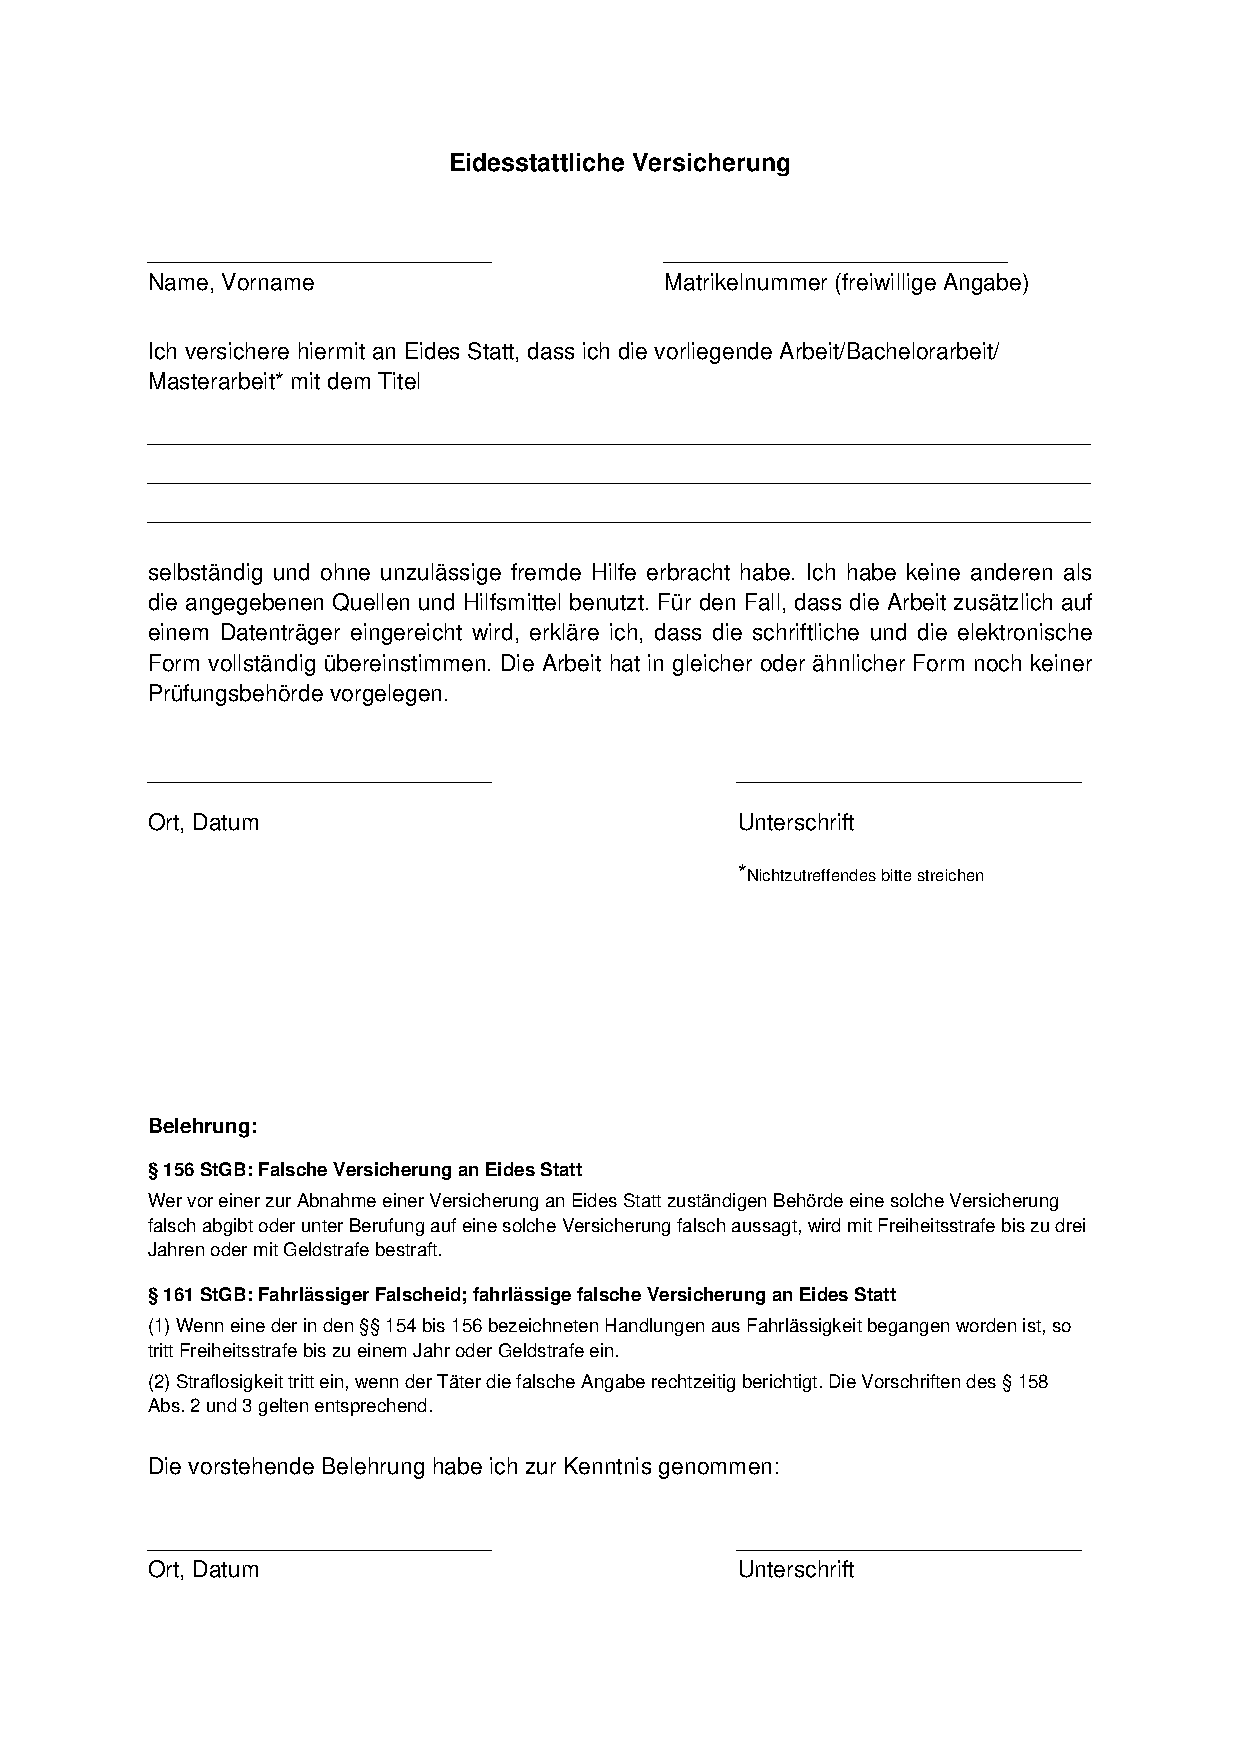
\includepdf[pages={1},offset=-1in -1in]{Formular_Eidesstattliche_Versicherung_neu.pdf}
% 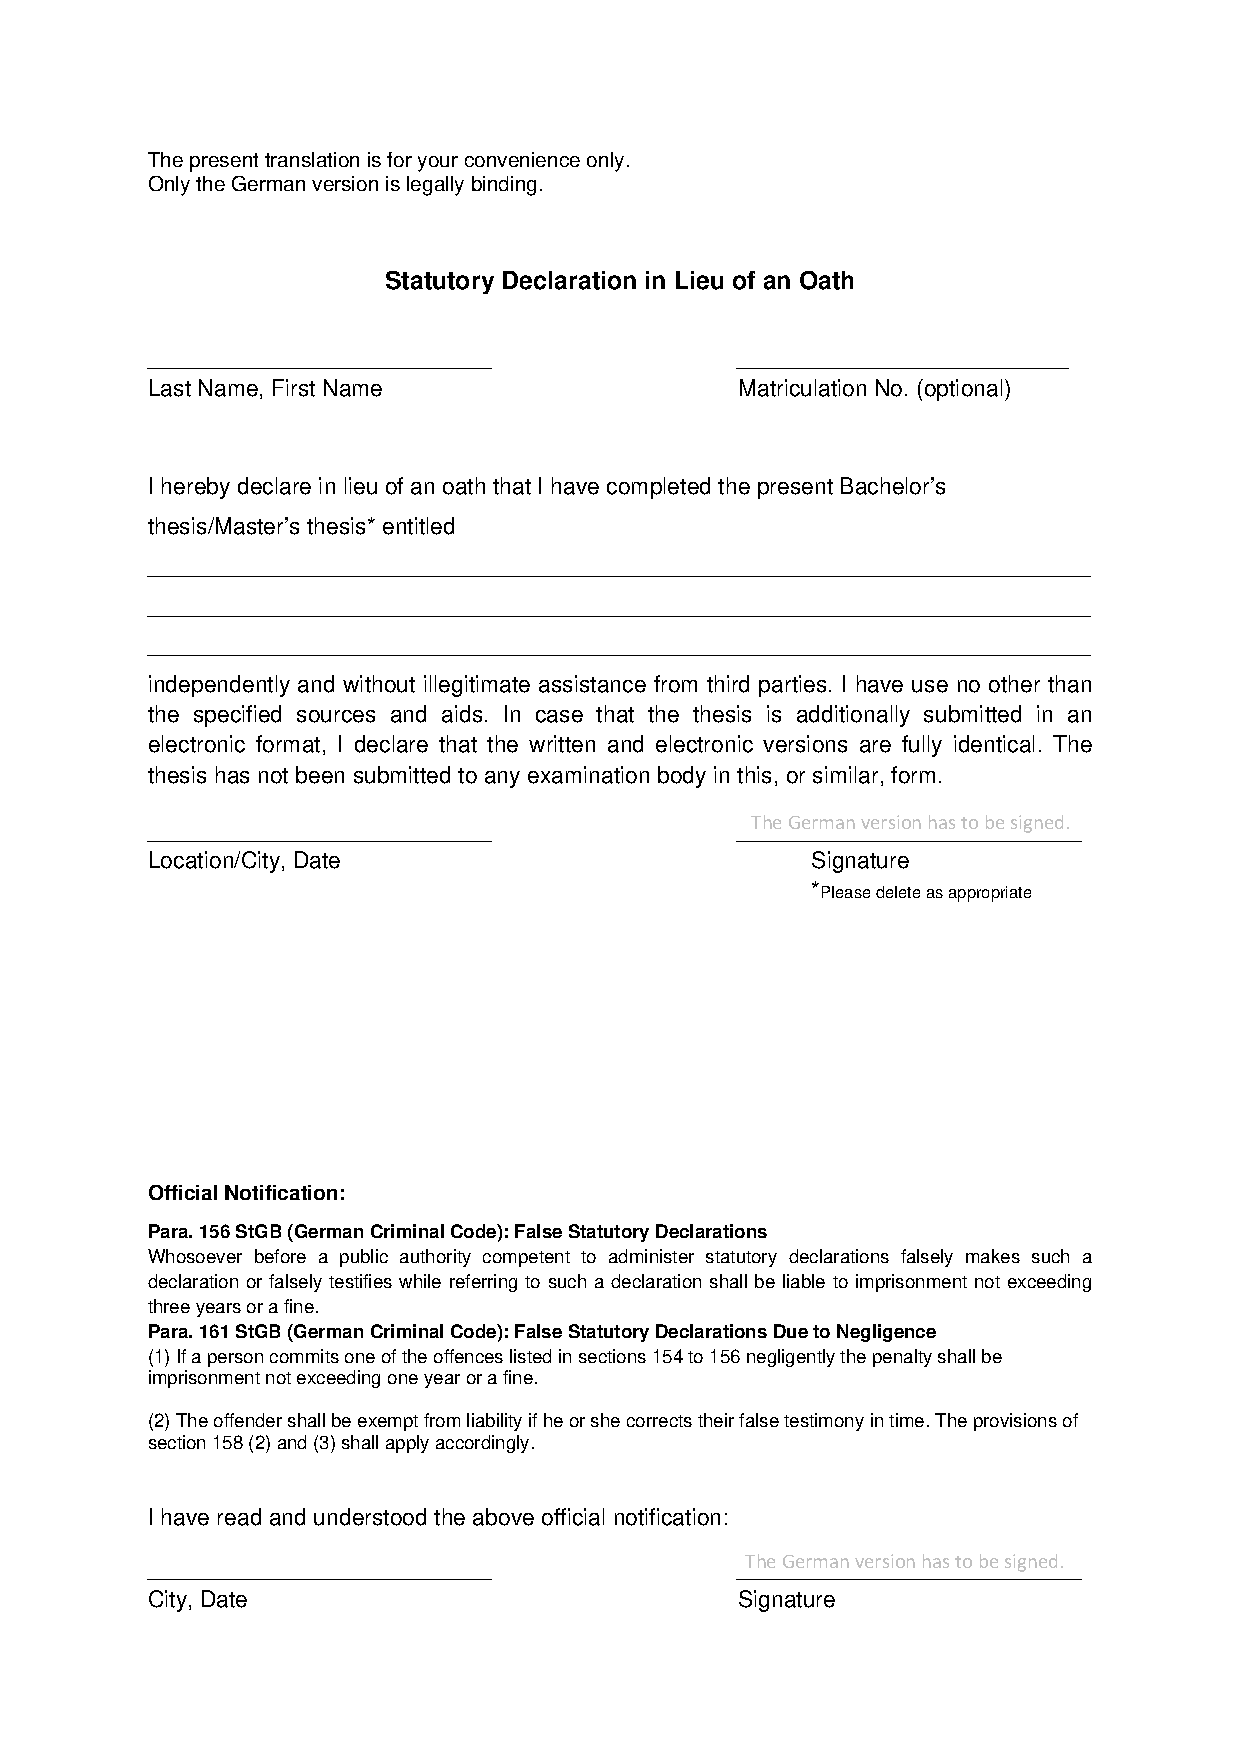
\includepdf[pages={1},offset=-1in -1in]{Statutory_Declaration_in_Lieu_of_an_Oath.pdf} % English 

\clearpage

{\bf\Large Abstract} \\ [1em]
The motivation of this paper is to introduce the sensor fusion and its significance in the improvement of object detection and sensing real-time environment. The first chapter of this paper explains the principal concepts, types and commonly used models of sensor fusion\cite{Wilfried2002}. The second chapter describes some real time applications of sensor fusion in the context of self-driving cars. Each application has different methodology. First, We will see the improvement of the perceived environment model for moving object detection and tracking by multiple sensor fusion where only front view point is considered \cite{Chavez_Garcia_2016}. After that we will explore another moving object detection and tracking experiment with sensor fusion where multiple sensors are configured in various view points of the vehicle which provides a very reliable and safety autonomous driving experience for real-world driving environments \cite{Cho_2014}. The next section describes an obstacle detection task which follows a robust sensor fusion-based method\cite{Shinzato_2014}. After that a sensor-independent fusion approach is described which allows effective sensor replacement and determine redundancy by using probabilistic and generic interfaces\cite{Kunz_2015}. This paper is not only limited to demonstrate the positive sides of sensor fusion, but also try to observe the limitations\cite{Wilfried2002}.

\input{src/tex/aufgabenstellung}

\tableofcontents

\clearpage

% Ab erstem Kapitel Seiten arabisch zählen
\setcounter{page}{1}
\pagenumbering{arabic}

\chapter{Introduction}

\section{Introduction}
Fusion techniques are very common in our nature. Animals sense the environment by eyes, ears etc. We, Humans, also have the ability to collect data about the environment model by five body senses. We can enrich the perceived environment model by combining all senses data \cite{Wilfried2002}. Like nature, science also adopt the fusion concept and successfully applied in its many fields. For example, self driving car needs to sense the environment by the sensors and sensor fusion helps to perceive the environment model more correctly. This paper tries to explain the basic concept of Sensor Fusion and also explains some of the applications of this concept.

\section{What is Sensor Fusion?}
The term \emph{Sensor Fusion} means fusing multiple sensor data to make a rich environment model. One sensor data may not cover all the information or in some cases one sensor may produces incomplete information. Fusion of multiple sensors data improves the quality of the data and produce more reliable environment model. According to \cite{Hall:2004:MTM:1204261} the term \emph{multisensor data fusion} defined as,
\theoremstyle{definition}
\begin{definition}{Multisensor data fusion}
is the technology concerned with the combination of how to combine data from multiple (and possible diverse) sensors in order to make inferences about a physical event, activity, or situation.
\end{definition}
On the other hand, the more formal definition of Sensor Fusion is defined in \cite{Wilfried2002} as,
\theoremstyle{definition}
\begin{definition}{Sensor Fusion}
is the combining of sensory data or data derived from sensory data such that the resulting information is in some sense better than would be possible when these sources were used individually.
\end{definition}
There is a confusion about \emph{multisensor integration} and \emph{sensor fusion}. In multisensor integration, data is received from multiple sensor but it is send to the control application directly without fusion. In sensor fusion, data also comes from multiple sensor but the control application get the fused data which is only one single representation of environment model and the control application gets only one data.

\section{Motivation for Sensor Fusion}
The following scenarios are very common whcih may fails physical sensor measurement\cite{Wilfried2002}:
\begin{description}
    \item[Sensor Element Broken:] A sensor is composed with some small elements. If one of the elements are broken, it would give incomplete results. Incomplete results would be produced for some other reasons, such as calibration issues,hardware malfunctions, uncertain detection and asynchronous scans, even from scene perturbations, like occlusions, weather issues and object shifting.
    \item[Only Covering Restricted Region:] An individual sensor has the capability of covering a limited range. For example, a camera sensor facing to the front side of a car could not cover the back side of the car.
    \item[Processing Time:] Some sensors are limited to processing power so that they need some time to capture and transmit the data. As a result, the frequency of measurement is also decreased. For example, a very complex camera sensor may sends the captured image of a pedestrian crossing the road after one or two seconds which is very risky for self driving car.
    \item[Uncertainty:] The single sensor measurement could be uncertain. For example, a distance sensor facing to the front of a car may capture the correct distance from a object or may be the sensor beam misses the object and giving the wrong distance. Actually, uncertainty occurs for missing functionality (e.g., occlusions) and also when sensor can not measure all relevant attributes of precept, or when the observation is ambiguous\cite{Wilfried2002}. Because of having coverage of limited region, a single sensor may produce uncirtain result\cite{Wilfried2002}.
\end{description}
Sensor Fusion could solves problems given above. The following advantages can be expected from sensor fusion over a single sensor\cite{Wilfried2002}:
\begin{description}
    \item[Robustness and reliability:] Depending on multiple sensor increase the redundancy of data and even if one of the sensors are broken, we expect accurate data.
    \item[Extended Coverage:] By multiple sensor, the environment can be observed from different faces and different angle.
    \item[Processing Parallel:] One sensor can take some time to process and other sensor can capturing and again when one finish processing start capturing and other stat processing.
    \item[Reduce Uncertainty:] Getting same data from multiple sensor reduce the uncertainty. For example, one sensor may miss the object but other may capture.
    \item[Prevent Interruption:] Using different types of sensors for same purpose can prevent interruption. For example, a self driving car is driving while raining and the camera sensor could not see the actual objects in-front of it because of rain drops. In this case, parallel performing an ultrasonic sensor can still measure the objects.
    \item[Improved Quality:] Getting same data from multiple source increasing the quality of the data.
\end{description}
One of the interesting advantage of sensor fusion is the possibility to reduce system complexity\cite{Wilfried2002}. It is possible to consider the sensor fusion component as a separate system and the main control system could communicate with it via defined interface. To do so we can modify the fusion subsystem without touching the main system\cite{Wilfried2002}.

\section{Categories of Sensor Fusion}
Sensor Fusion is categorized by different applications in aspects. In the following parts, the categories are described.

\subsection{Three-Level Categorization}
According to level of data the fusion process can be categorized by following criteria:
\begin{description}
    \item[Low-level fusion] is also known as \emph{raw data fusion} refers to fusion of raw data from multiple sensor and combine them to produce new data which is more reliable and understandable than the raw data.
    \item[Intermediate-level fusion] is also knows as \emph{feature level fusion} refers to collecting a bunch of features and keep the features into a feature map which can be used by AI applications like segmentation and detection of objects. For example, keeping features like edges, corners, lines are useful for pedestrians detection.
    \item[High-level fusion] is also known as \emph{decision fusion} refers to making decisions from several sensors. For example, voting, fuzzy-logic and statistical methods.\cite{Wilfried2002}.
\end{description}

\subsection{Categorization Based on Input/Output}
Dasarathy extend the three-Level categorization based on input/output\cite{Wilfried2002}. Actually if the input output are considered then the input of one level comes from another level. For example, the input of feature extraction comes from raw data and the raw data produce selection of some features. So, the levels are not same anymore.  In Figure \ref{fig:InputoutputCat}, the relation between three-Level categorization and input/output is shown.
\begin{figure}
  \centering
  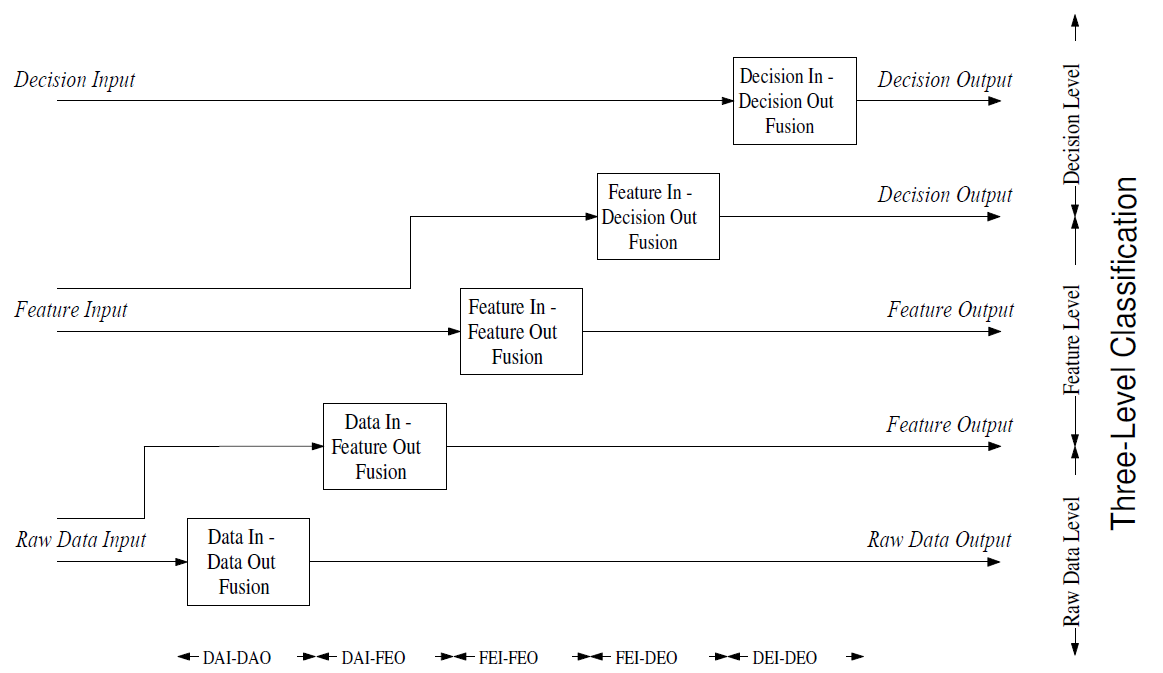
\includegraphics[width=1.1\textwidth]{src/pic/InputoutputCat.png}
  \caption{Fusion Categorization by input/output}
  \label{fig:InputoutputCat}
\end{figure}

\subsection{Categorization Based on Sensor Configuration}
Sensor fusion may be in different configuration types. According to various configuration, sensor fusion can be categorized into three sections\cite{Wilfried2002}:
\begin{description}
    \item[Complementary:] A configuration is considered as a complementary configuration when the sensors participating in sensor fusion are not directly dependent on each other, but it would be a case where inputs of the sensors are mixed to produce complete result. This configuration solves on of the common problem of single sensor system which is incompleteness of sensor data.
    \item[Competitive:] Competitive configuration can be achieved by keeping multiple sensors for observing same object or view which are independent from each other. This configuration ensure high redundancy of data and that is why it is also called \emph{redundant configuration}\cite{Wilfried2002}.
    \item[Cooperative:] A cooperative mechanism is the intelligent one in a sense that in this configuration the inputs from separate sensors are combined to produce a information which is not available in the single sensor inputs. An example for a cooperative sensor configuration is stereoscopic vision - by combining two-dimensional images from two cameras at slightly different viewpoints a three-dimensional image of the observed scene is derived\cite{Wilfried2002}.
\end{description}

There could be more categories exists but commonly used sensors are categorized like above. 

\section{Commonly used Sensor Fusion Models/Applications}

\subsection{Evidential Framework}
The Evidential framework is a generalization of the Bayesian framework of subjective probability\cite{Chavez_Garcia_2016}. Evidential theory (ET) is applicable to the problems which are ambiguous and unpredictable for finding solutions. We can apply it on uncertain problems to have a belief based on available proofs. There are two major concepts, mass function and belief function to perform uncertainty reasoning\cite{Bell_4028391}.\\
Assume, $\Omega$ is a set of hypotheses over a hypothesis space. A function $m:2^\Omega \rightarrow[0, 1]$ is called mass function which is defined as follows\cite{Bell_4028391}:
$$M1. m(\emptyset)=0$$
$$M2.\sum_{x \subseteq \Omega} m(X) = 1$$
where, $\emptyset$ is an empty set, $X$ is a variable and the assigned uncertainties are called $m-$values\cite{srivastava2011introduction}. For the variable $X$, we can have $m(x) \geq 0$, $m(\neg x) \geq 0$, and $m(\{x,\neg x\}) \geq 0$, such that $m(x) + m(\neg x) + m(\{x,\neg x\}) = 1$\cite{srivastava2011introduction}. We can have $m-$values for all the subsets of single element, double element, triple element and so on over the a hypothesis space and this hypothesis space contains all probable values of variable $X$. For example, a proof $Pr_{1}$ is $m_{1}(x)=0.8$, $m_{1}(\neg x)=0.15$ and $m_{1}(\{x,\neg x\}) = 0.05$. It means $80\%$ agree that $X$ is $\mathbb true$, $15\%$ agree that $X$ is $\mathbb false$ and $5\%$ are not sure reflecting ignorance.\\
Another function $bel:2^\Omega \rightarrow[0, 1]$ is called belief function which is defined as follows\cite{srivastava2011introduction}:
$$bel(O) = \sum_{C \subseteq O} m(C)$$
where, $O$ is a set of elements which is the summation of all $m-$values of that set of elements denoted by $C$. As like probability theory it is not needed  to be $1$ the summation of belief in $O$ and belief in $\neg O$ which is actually less or equal to $1$, i.e., $bel(O) + bel(\neg O)\leq 1$\cite{srivastava2011introduction}. Zero belief, i.e., $bel(x) = 0$, and $bel(\neg x) = 0$ indicates the lack of proofs, also in other other word it indicates ignorance. For example, again consider the previous example $Pr_{1}$. In this case, $bel_{1}(x) = m_{1}(x) = 0.8$, $bel_{1}(\neg x) = m_{1}(\neg x) = 0.15$ and $bel_{1}(\{x, \neg x\}) = m_{1}(x) + m_{1}(\neg x) + m_{1}({x, \neg x}) = 0.8+0.15+0.5 = 1$.\\
The fundamental operation of evidential reasoning is the orthogonal sum of evidential function (mass and belief function), which is known as Dempster's rule for combining proofs\cite{Bell_4028391}. The Dempster's rule to combine $m-$values can be written as (Shafer 1976) follows\cite{srivastava2011introduction}:
 $$m(O \neq \emptyset) = \frac{1}{k}  \sum_{O=C_{1} \cap C_{2}} m_{1}(C_{1})m_{2}(C_{2})$$
where, $K$ is the renormalization constant and 
$$K = \sum_{C_{1} \cap C_{2} \neq \emptyset} m_{1}(C_{1})m_{2}(C_{2}) = 1-\overbrace{ \sum_{C_{1} \cap C_{2} = \emptyset} m_{1}(C_{1})m_{2}(C_{2})}^{CV}$$
$CV$ in $K$ indicates the conflict value which is distributed among all the elements of the frame of discernment\cite{Chavez_Garcia_2016}.\\
Generally, ET considers three situations, $\mathbb true$, $\mathbb false$ and not sure (ignorance) by which it can find solutions for ambiguous and unpredictable problems more powerfully. For example, an online shop's admin wants to know the degree of satisfaction for a delivered product $A$ from the customers. The answer from customer $C_{1}$ is $80\%$ satisfied, $15\%$ unsatisfied, $5\%$ not sure. Answer from another customer $C_{2}$ is $60\%$ satisfied, $20\%$ unsatisfied, $30\%$ not sure. Assume, a hypothesis space is, $\Omega = \{S, U\}$ where $S$ and $U$ stand for satisfiability and unsatisfiability respectively. So, we have two set of proofs for $C_{1}$ and $C_{2}$. According to ET, the combination of two proofs can be represented in Table \ref{table:customer_surv} \cite{Bell_4028391}.
\begin{table}[]
\centering
\caption{Combination of two customer surveys}
\label{table:customer_surv}
\begin{tabular}{|l|l|l|l|}
\hline
 $m^{\prime}=C_{1}\oplus C_{2}$&  $m_{1}(S)=0.8$ & $m_{1}(U)=0.15$ & $m_{1}(\{S, U\})=0.5$ \\ \hline
 $m_{2}(S)=0.6$& $0.8x0.6=0.48$ & $\emptyset$ & $0.6x0.05=0.03$ \\ \hline
 $m_{1}(U)=0.2$& $\emptyset$ & $0.2x0.15=0.03$ & $0.2x0.05=0.01$ \\ \hline
 $m_{1}(\{S, U\})=0.3$& $0.3x0.8=0.24$ & $0.3x0.15=0.045$ & $0.3x0.05=0.015$ \\ \hline
\end{tabular}
\end{table}
By applying Dempster's rule, we get as follows:
$$K = \sum_{C_{1} \cap C_{2} \neq \emptyset} m_{1}(C_{1})m_{2}(C_{2}) = 1- \sum_{C_{1} \cap C_{2} = \emptyset} m_{1}(C_{1})m_{2}(C_{2})$$
$$=0.48 + 0.03 + 0.03 + 0.01 + 0.24 + 0.045 + 0.015 = 0.85$$
$$m^{\prime}(S)=(\frac{1}{0.85})(0.48 + 0.03 + 0.24) = 0.882$$
$$m^{\prime}(U)=(\frac{1}{0.85})(0.03+0.01+0.045) = 0.1$$
$$m^{\prime}(\{S, U\})=(\frac{1}{0.85})(0.015) = 0.017$$
So, the combination result is $88.2\%$ satisfied, $10\%$ unsatisfied and $1.7\%$ undecided. Authors has used this evidential approach based on mass distributions over the set of different class hypotheses\cite{Chavez_Garcia_2016}.

\subsection{Kalman Filter}
The Kalman Filter(KF) is a linear mathematical model which uses a recursive algorithm for fltering signals by measuring a respectable amount of statistical and systematical errors[1]. It was developed by Kalman and Bucy in 1960[1].KF generates a estimation of the true and measured values[2]. First, it predicts a value. Then it measures the ambiguity of previous value. Finally, it performs an weighted average of both the predicted and measured values[2].
The more the weight is, the less the ambiguity is. The output of a KF is the estimation which is closer to true values. This is the basic operation of a KF.\\
A standard KF model is explained by two linear equations[1]. The first equation measures the state of a system at time $k$ which is governed by the linear stochastic difference equation[2]:
$$aaa$$
\begin{table}[!htbp]
\centering
\label{my-label}
\begin{tabular}{llll}
where, & $bbb$     & = & a vector representing the state at time $k-1$                                                                                                                                         \\
       & $A$       & = & non singular state transition matrix                                                                                                                                                  \\
       & $ccc$     & = & a vector representing the input of the system at time $k-1$                                                                                                                           \\
       & $B$       & = & The relation between $bbb$ and $ccc$                                                                                                                                                  \\
       & $w_{k-1}$ & = & a random variable representing the process noise, \\
       &        & & modelled as white noise $\sim N(0; Q)$, where $Q$ is the covariance matrix
\end{tabular}
\end{table}\\
with a measurement which is the second equation[2]:
$$eee$$
\begin{table}[!htbp]
\centering
\label{my-label}
\begin{tabular}{llll}
where, & $fff$     & = & a vector representing the sensor observation at time $k$                                                                                                                                         \\
       & $H$       & = & a matrix relates the measurements to the internal state                                                                                                                                            \\
       & $v_{k}$ & = & a random variable representing the measurement noise, \\
       &        & & also modelled as white noise $\sim N(0; Q)$, where $R$ is the covariance matrix
\end{tabular}
\end{table}

\subsubsection{Kalman Filtering Algorithm}
To start a KF, user has to give an estimation $lll$ and an estimate of its covariance $P_{0|0}$ i.e., inaccurate start value. After initialization user can traverse the Kalman Filtering Algorithm. It has following steps[1]:
\begin{enumerate}
  \item  Compute a predicted priori state estimation of state $xxx$ at time $k$ by using given observations up to $k-1$.
  $$ggg$$
  \item Compute predicted error covariance matrix at time $k$.
  $$hhh$$
  \item Compute Kalman gain.
  $$iii$$
  \item Update the estimation by a measurement $z_{k}$.
  $$jjj$$
  \item Update error covariance matrix.
  $$kkk$$
  where, $I$ is the identity matrix.
\end{enumerate}

After performing these 5 steps the iteration restarts again from step 1, but with $k:=k+1$.\\
So, we can say that The equations containing in the steps of above algorithm can be divided into two groups: time update equations (equation 1 and 2) and measurement update equations(equation 3-5)[3]. Also the final estimation algorithm looks like  a predictor-corrector algorithm as shown in Figure [cycle].

\subsubsection{Underlying Dynamic System Model}
KF is based on linear and non-linear dynamical systems discretized in the time domain[3]. As shown in Figure [underlying], each state represents a real vector and a sequence of noisy observations are the inputs of internal states. The system is modeled according to the state space representation of the KF specifying the matrices i.e., the state transition model ($A$), the observation model ($H$), the covariance of the process noise ($Q$), the covariance of the measurement noise ($R$), and sometimes the control-input model ($B$) for each time-step $k$.\\
There are lot of dynamic systems which do not support KF as it is a linear model[2]. To deal with these type of dynamic systems Extended KF and Unscented KF are used which are the extended version KF[2].

\chapter{Applications}

\section{Applications}
In the current age, Sensor fusion are used in the systems which were only found in science fiction books and was just an imagination (e.g. self driving car). It has become the key component for moving object detection and tracking\cite{Cho_2014, Chavez_Garcia_2016}, obstacle detection\cite{Shinzato_2014} which are the most challenging task in the application domain of autonomous driving cars. In the following parts of this paper, some of the successful application of sensor fusion is described.


\section{Multiple Sensor Fusion for Moving Object Detection and Tracking}
The intelligent vehicles are now becoming capable of instruct themselves to drive in very dynamic and unstructured environment. But driving in such an environment increase uncertainty. One of the uncertain task is to moving object detection and tracking. Perceiving the environment involves the selection of different sensors to obtain a detailed description of the environment and an accurate identification of the objects of interest\cite{Chavez_Garcia_2016}. So, Fusion of multiple sensor could decrease the uncertainly in moving object detection task. In the following, two different approaches are described for moving object detection which are different in the view point of the sensors.

\subsection{Front View Approach}
In \cite{Chavez_Garcia_2016}, an advanced driver assistance systems (ADAS) is introduced which main task is to help the drivers to avoid dangerous situations. ADAS assists with warning messages in dangerous driving situations (e.g., possible collisions), activation of safety devices to mitigate imminent collisions, autonomous maneuvers to avoid obstacles, and attention-less driver warnings\cite{Chavez_Garcia_2016}. There are two major tasks to perceive the environment. The task simultaneous localization and mapping (SLAM) is one of and another one is to detect and track the moving objects (DATMO). The model of perception task is shown in figure \ref{fig:datmoslam}.
\begin{figure}
  \centering
  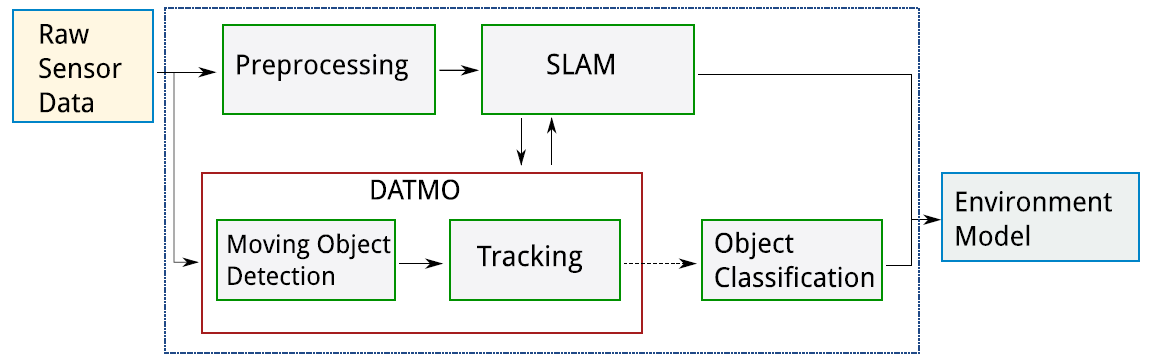
\includegraphics[width=.6\textwidth]{src/pic/datmo_slam_arch.png}
  \caption{General Architecture of perception task. \cite{Chavez_Garcia_2016}}
  \label{fig:datmoslam}
\end{figure}
\begin{description}
    \item[SLAM:] could be defined as follows. A self driving car is moving in an unknown environment and it starts moving from a known location. Meanwhile, it's motion is uncertain which makes the determination of it's global position more difficult. As it is moving, continuously it perceives the environment. In this situation, SLAM is the procedure of building a map of the environment while simultaneously calculating the cars position relative to the map\cite{Thrun2008}. More formally we can say, the SLAM problem asks if it is possible for a autonomous agent to move to an unknown location in an unknown, dynamic or unstructured environment and for the agent to incrementally build a consistent map of this environment while simultaneously determining its location within this map\cite{Bailey:1638022}.
    \item[DATMO:] While SLAM creates a map of static objects including the position of the agent, DATMO uses the map  of static objects generated by SLAM \cite{Azim:6232303} to determine the object to be moving or static\cite{vu2008mapping}. On the other hand, by perform DATMO it is possible to get the position of moving objects around, track them and even predict the future behaviour of those moving objects\cite{vu2008mapping}.
\end{description}

It is assumed that the SLAM is a solved task. As a result it is more reasonable to focus on the DATMO\cite{Chavez_Garcia_2016}. DATMO is performed with an Evidential fusion approach where object classification is the key component. Additionally, Evidential fusion handle uncertainty of sensor detection. Actual goal is to find a list of moving objects with their velocity which should improves the ADAS.

Handling incomplete environment data is one of the important factor of assistance systems which leads to wrong perception. The reasons for incomplete sensor data are already described in the introduction section of this paper. Including incomplete information, there is another problem exists in the tracking process. The tracking process expects that all inputs are moving objects. But in the real world, environment consists of both moving and static objects. So, moving object detection is a very difficult task of moving object tracking system and various number of sensors need to work together to perform the task.

\subsubsection{Environment Setup}
In the experiment \cite{Chavez_Garcia_2016}, a Lancia Delta car is decorated with necessary equipment such as a processing unit for processing the image and create moving object list, some components which is responsible for driver interaction and the front - facing sensors i.e., Lidar, Camera and Radar. So the sensors only cover the front view of the vehicle as shown in figure \ref{fig:sensorcovarage}. An IBEO Lux laser scanner is used as the lidar sensor which can deliver a 2D list of impact points and it can cover all the points in the range of 200m. The radar is used to detect moving targets. It could detect targets within 150m and the velocity range up to 250kph. The camera would capture black and white images.

\subsubsection{System Architecture}
The fusion process is performed in a Perception System (PS) which is developed according to improve the efficiency and increase the quality of sensor data. It tries to concentrate on object detecting and tracking to improve the data quality. The PS aims at detecting, classifying and tracking a set of moving objects of interest that may appear in front of the vehicle\cite{Chavez_Garcia_2016}. The structure of the  PS is shown in Figure \ref{fig:PS}. In this system, the fusion module is taking input directly from the three sensors. Initially lidar, radar and camera get the input from the environment and create a list of detected objects for each sensor. Those three lists are then provided to the fusion module. Each environment object is demonstrated by their position, size and evidence distribution of class hypotheses. On the other hand, classifications are done by the shape, relative speed and visual appearance of the detected objects. Precisely, the lidar and radar is performing the task of detection while camera is extracting the features of the detected objects to classify them. The fusion module fused the three list of objects and combined them into one list  where each object contains combined description. The ultimate output of the fusion method is provided to the tracking module to calculate the moving objects states which is actually the final output of the DATMO task. Three sensors are contribution in the task of moving object detection and tracking. The next sections are going to describe briefly how the the sensors prove information for detection and tracking.

\begin{figure}
    \centering
    \begin{subfigure}[b]{0.4\textwidth}
        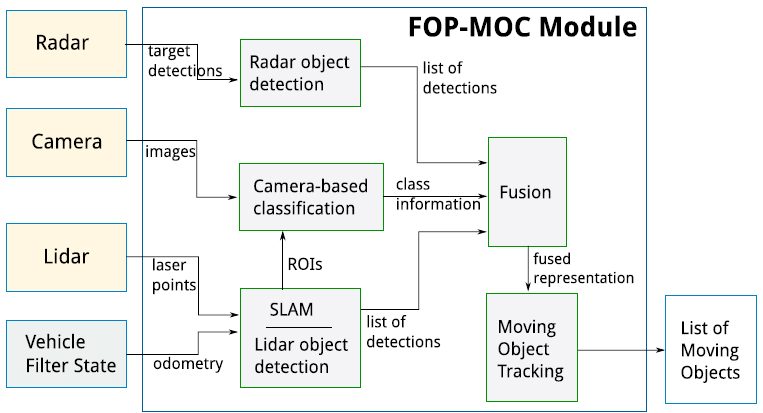
\includegraphics[width=\textwidth]{src/pic/PS.png}
        \caption{}
        \label{fig:PS}
    \end{subfigure}
    \begin{subfigure}[b]{0.4\textwidth}
        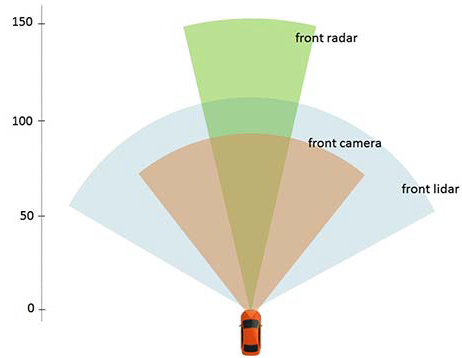
\includegraphics[width=\textwidth]{src/pic/sensor_covarage_front.png}
        \caption{}
        \label{fig:sensorcovarage}
    \end{subfigure}
    \caption{\ref{fig:PS}:Sensor Fusion model, \ref{fig:sensorcovarage}:Coverage of the sensors}
    \label{fig:group1}
\end{figure}

\subsubsection{Moving Object Detection}
The process of three individual sensors for Moving object detection are described bellow:
\begin{description}
    \item[Lidar Processing:] Lidar is used as the leading sensor in the setup as it can produce high resolution data with more accurate result. The principal task of lidar is to get exact information of the shape of the moving object in front of the vehicle. Though the main pourpose is to focus on DATMO task, the SLAM component is also implemented to get the map of objects and vehicles position in the map\cite{Chavez_Garcia_2016}. By the lidar data a 2D Bayesian occupancy grid map is created. Each cell in the map is filled with or not by an object where vehicles location if found by Maximum Likelihood approach. Each time the sensor updates, the map is recalculated and the vehicle position is also re-estimated. Besides, lidar based detection also works with the help of the grid map. If the a cell of grid map is occupied with an obstacle which was previously free cell, then it is said to be a moving object. In the contrast, if a cell is occupied with an object which was also previously occupied, then it is said to be a static object. The SLAM process is completely independent from the moving object detection task.
    \item[Camera Images:] The camera images are processed to extract the visual features and classification.
    \begin{enumerate}
        \item{Visual Representation:} The Histograms of Oriented Gradients (HOG) descriptor is taken as the core of vehicle and pedestrian visual representation as it has already shown promising results\cite{Chavez_Garcia_2016}. The main goal is to extract the graphical details of the particular area of the image which is important to extract for future use to find out the existence of the object of interest. A sparse version of the HOG descriptor (S-HOG) is proposed to use instead of actual HOG descriptor which focuses on specific areas of an image patch \cite{Chavez_Garcia_2016}. S-HOG reduces the common high-dimensional HOG descriptor to explains the selected block of the image of different class.
        \item{Object Classification:} Detecting the region of interest (ROI) from camera image is a performance degrading task. On the other hand, the ROI is already available from lidar sensor and that is why already provided ROI is used in the camera images to specify object region. Every ROI is processed to extract the visual features and a classifier is applied to decide if an object of interest is inside the ROI. As the speed and quality of the result is totally depend on the choice of the classifier, an optimized and boosting-based learning algorithm is implemented which is called discrete Adaboost\cite{Chavez_Garcia_2016}. This algorithm combines many week classifiers and combine them to make the powerful one which increase the performance. For each class of interest e.g., pedestrian, bike, car, truck, a binary classifier was trained off-line to identify object (positive) and non-object (negative) patches\cite{Chavez_Garcia_2016}.
    \end{enumerate}
    \item[Radar Targets:] Radar sensor has a build in method to detect moving objects. Radar creates a list of n moving objects and send the list to perception approach. Each element of the list contains the range, direction of moving and relative speed of the detected target. There are some limitation of Radar sensor. One problem is, Radar also could include static objects in the list. Sometimes the week objects could not always detected by the Radar which leads to miss detection. Because of various problems, the targets are tracked using constant velocity, acceleration and turning models represented by Interactive Multiple Model (IMM).
\end{description}

\subsubsection{Moving Object Classification}
The information about kinetic state of the objects with classification is determined in detection level. The descriptions found from detection level is very useful for better estimation of object's motion and removes number of miss leading detection. In detection level, only one class is selected for the object which means it is not possible to fix the classification if the initial one is wrong. It is necessary to keep more than one approximate classifier so that in case of wrong classification, it is easy to get the correct classifier.

A composite representation is formed by two parts: kinetic + appearance\cite{Chavez_Garcia_2016}. Kinetic description includes position and shape information in a 2D space. Appearance description includes an evidence distribution m($2^{\Omega}$) for all possible class hypothesis where $\Omega$= \{pedestrian, bike, car, truck\} is the frame of discernment representing the classes of interest\cite{Chavez_Garcia_2016}. The fusion module mainly detect and track the objects in the from of $\Omega$ and perform the classification. The process of three individual sensors for Moving object classification are described bellow:
\begin{description}
    \item[Lidar Sensor:] In the detection task, the shape of the moving object is already found. So, the shape of the object can be used for kinetic representation. The modeling of the moving objects are done by a box \{x,y,w,l,c\}, where x and y are the center of the box, w and l are the width and length according to the class of object \cite{Chavez_Garcia_2016}. But if the moving object is very small, the box model doesn't fit. For example pedestrians are not able to modeled by a box rather it is assume to be a 2D object. So for small objects a point model \{x,y,c\} is suited well where x, y are the 2D coordinate of center of the object and c is the class. Classification of objects is done based on the shape and size of the object which follows a fixed fitting-model approach. It is hard to get the exact classification of moving object because the visibility is temporary. For example, if the width of an object in less than a threshold, it is classified as a bike or pedestrian.
    
    In this way, it is necessary to know the threshold for all classes. The thresholds are defined for examining the size of typical passenger cars, trucks and motorbikes sold in Europe\cite{Chavez_Garcia_2016}. In this experiment, instead of keeping only one class decision, a basic belief assignment $m_{1}(A)$ for each $ A \in \Omega $ is defined, which describes an evidence distribution for the class of the moving object detected by lidar\cite{Chavez_Garcia_2016}.
    \item[Camera Sensor:] In the detection phase, lidar provides a set of ROIs which are used to generate hypothesis that the objects are located in the image at the place of the set of ROIs. To verify the hypothesis, off-line classifiers are applied to classify different objects. The camera image classification extracts more information from a ROI by dividing the ROI into several sub regions. After classification of each ROI has done, a belief assignment $m_{c}$ is calculated which represents the evidence distribution for the classes hypotheses\cite{Chavez_Garcia_2016}.
    \item[Radar Sensor:] This sensor is mainly used for moving object detection. But if other sensors can not classify then this sensor tries to classify moving objects. As radar can determine the speed, speed is used for classification. The slowest speed of the vehicle classes is estimated statistically and determine a threshold for each class. That means for cars, trucks, bikes and pedestrians there is a threshold and if the moving object move in a speed of the threshold than the object classified as the corresponding class. Finally, the basic belief assignment is calculated based on the speed classification\cite{Chavez_Garcia_2016}.
\end{description}

\subsubsection{Sensor Fusion}
Once the DATMO and object classification task is finished, the composite object representation are ready for fusion. A multi-sensor fusion framework is proposed at the detection level which not only depend on three sensors but also many sensors can be added to the framework to extend the fusion process\cite{Chavez_Garcia_2016}. The combination of different representation of same object at detection level increase the reliability and reduce incompleteness, uncertainty of the detection result. For fusion approach it is important that for example an object getting from three sensors are same or are associated with each other. If an object $i$ is detected in sensor $a$ and $b$ and the detected objects are presented as $a_{i}$ and $b_{i}$ respectively. After detection the following things can be happen,
\begin{itemize}
    \item $a_{i}$ and $b_{i}$ are the same object; i.e., P($a_{i}$, $b_{i}$) = 1
    \item $a_{i}$ and $b_{i}$ are not the same object; i.e., P($a_{i}$, $b_{i}$) = 0
    \item ignore the association; i.e., P($a_{i}$, $b_{i}$) = $\Omega$
\end{itemize}

The object associations can be calculated by finding the similarity measures between them. Sensor $a$ and $b$ could provide different kind of description about the object. The description could be the position, shape or appearance information such as class. The similarity can be calculated based on the position or appearance information of the detected object. After two objects are decided to be same, the fusion method combines the object representation by fusing the information received from multiple sensors\cite{Chavez_Garcia_2016}. The fused object with kinetic and appearance information, are passed to the tracking system to estimate object motion model. The objects, for which no association is found, are simply removed by the tracking process.

\subsubsection{Experimental Outcome}
The perception System (PS) is tested in both highway and urban area with high traffic scenarios. In both areas, all vehicles including coming ones, are detected and tracked\cite{Chavez_Garcia_2016} as shown in figure \ref{fig:Experimental_PS}. Another good thing is that it could found out the static objects as well. From the figure. \ref{fig:Experimental_PS} it is shown that the vehicle speed are also detected. It is possible only because of fused information. Radar providing the speed and direction of the vehicle where lidar gives shape information and camera gives more detailed image description like hand or leg of a pedestrian. The class of object is improved by fused information from the three different sensors.
\begin{figure}
  \centering
  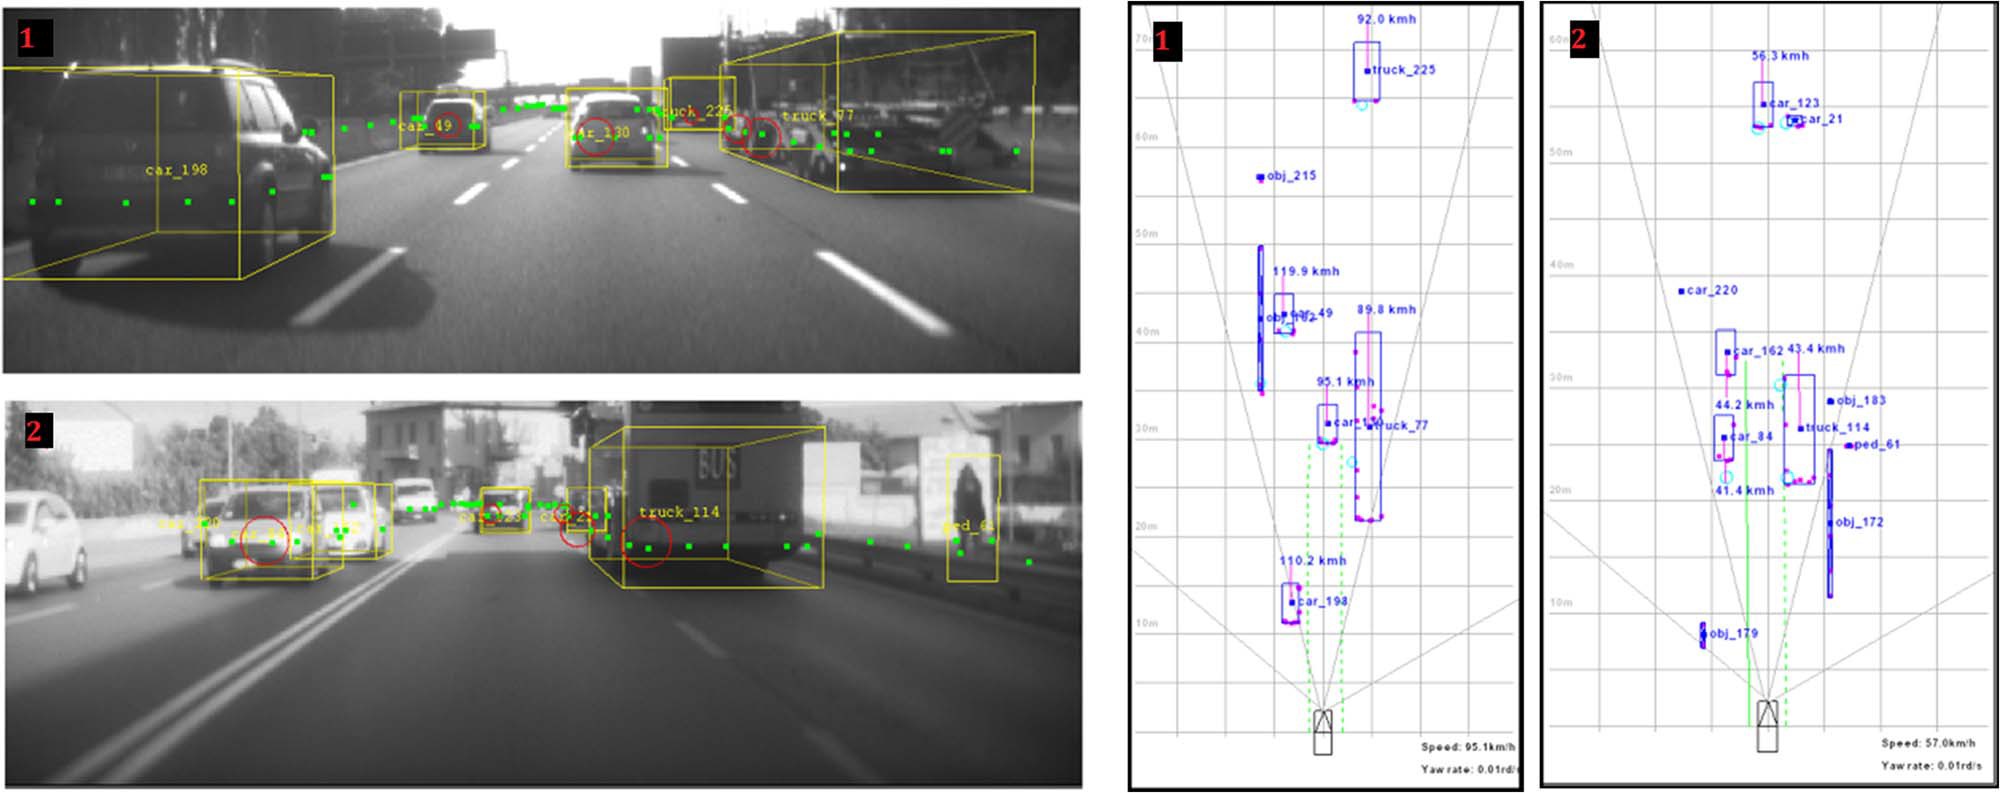
\includegraphics[width=1\textwidth]{src/pic/Experimental_PS.png}
  \caption{Results of PS 1: Highway, 2: Urban Areas \cite{Chavez_Garcia_2016}}
  \label{fig:Experimental_PS}
\end{figure}

\subsection{Multiple View Approach}
In \cite{Cho_2014}, a previously build perception system is improved to adopted the real world driving experience. The previous perception system was designed for a robotic vehicle which could operated on a simple, urban environment setup having no obstacle objects with limited vehicle interactions \cite{Cho_2014}. But in the real world, an autonomous driver agent have to be aware of all possible risky situations such as prevent coalition with nearby pedestrians or vehicles. To have safety driving experience, it is very obvious to detect and track the moving objects. In this paper\cite{Cho_2014}, the previously developed perception system and the moving object tracking system are redesigned to ensure the safety and reliability. Even new sensors are placed in different view of the vehicle.


\subsubsection{Environment Setup}
The sensors are configured in a vehicle in a manner to track all the moving objects, cover the region around the vehicle within a certain range and take advantage of vehicle's build in sensors. According to those criteria the sensors are placed like shown in Figure \ref{fig:Sensor_Setup_Multiple_View} (a). All the sensors are set in the vehicle body in a way that the sensors are not visible from outside. Precisely, six radars, six LIDARs and three cameras are installed in the experiment vehicle. One radar is paired with a LIDARs at different height. Robust number of sensors are used to get maximum reliability with an extended range of sensor coverage. According to \cite{Cho_2014} the current setup, any object which exists in the range of 200 meters of the vehicle can be observed by any of the sensors. Any object in the range of 60 meters could be observed by at least two sensors either radar and LIDAR or radar and camera. The coverage of sensors are visualized in the Figure \ref{fig:Sensor_Setup_Multiple_View}(b). There are three cameras in three different-looking faces. One camera is installed in froward facing approach inside the front window. Another camera is installed in the rear bumper to provide the front and back side of perspective images. The third one is a thermal one which is able to sense even in night or foggy weather. Another advantage of having wide range of sensors is that the spots are small enough that no vehicle will be overlooked\cite{Cho_2014} Overall there are 14 sensors are installed in the vehicle.

\begin{figure}
  \centering
  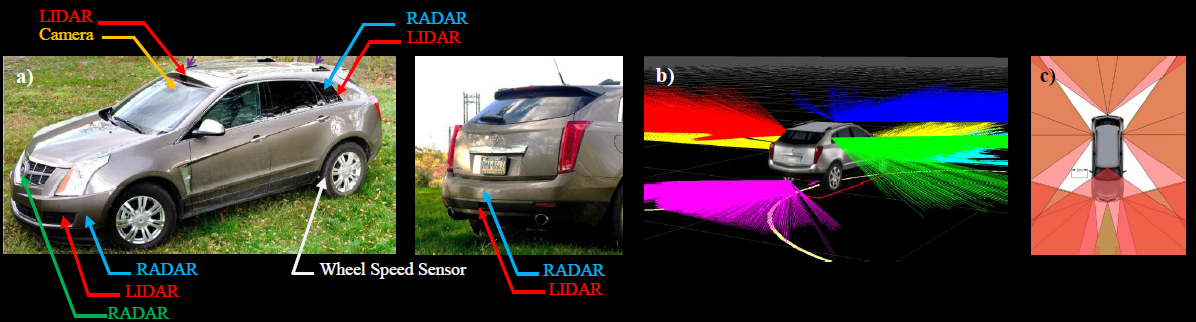
\includegraphics[width=1\textwidth]{src/pic/Sensor_Setup_Multiple_View.png}
  \caption{\cite{Cho_2014}}
  \label{fig:Sensor_Setup_Multiple_View}
\end{figure}

\subsubsection{System Architecture}
\begin{figure}
  \centering
  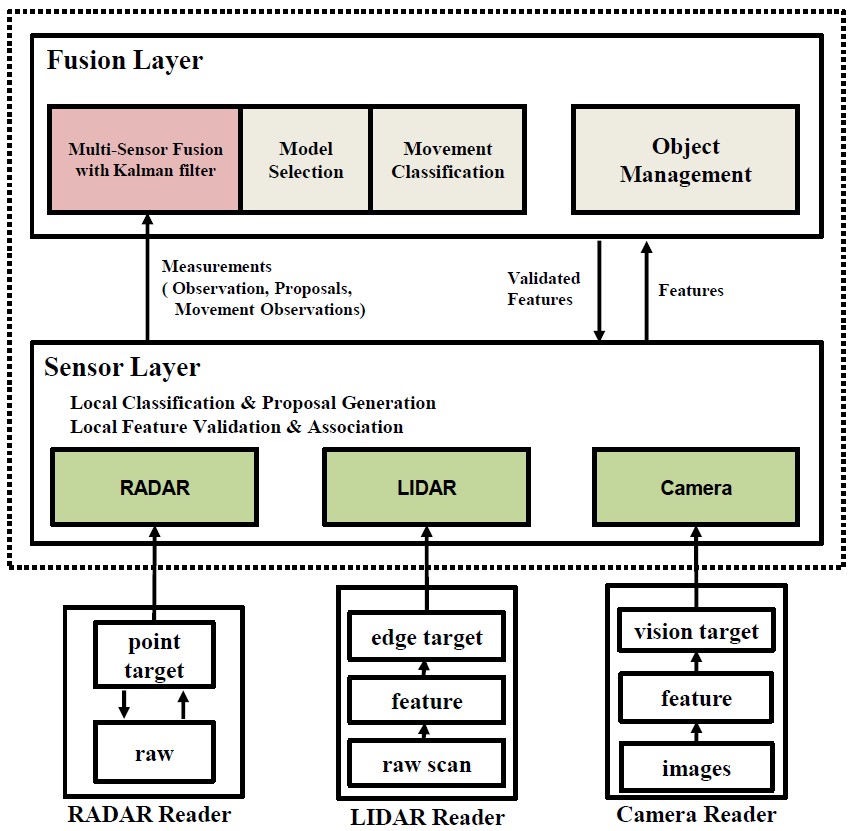
\includegraphics[width=.6\textwidth]{src/pic/Fusion_Arch_Multiple_View.png}
  \caption{\cite{Cho_2014}}
  \label{fig:Fusion_Arch_Multiple_View}
\end{figure}
The new redesigned perception system have two parts i.e., sensor and fusion layer as shown in figure \ref{fig:Fusion_Arch_Multiple_View}. Dividing the system into two independent module makes it possible to develop them independently based on an interface without knowing each others internal functionality. There is a common communication channel available for data exchange between those two modules. Each time new raw sensor data is available, reader extract features such as lines or corners and push the data to the common communication channel. The shared data is accessed any time by the higher level module i.e., fusion module. In fusion layer, the sensor measurements are processed as unit of measures where each object measured as a box model, but they are presented differently\cite{Cho_2014}. For example, a radar provides 2D position and velocity of an object. Radar data is represented in an array where time as the index of the array. Radar measurement in $k^{th}$ second  is:
\begin{equation}
z^{R}(k) = \{r_{1},r_{2},...,r_{p}\} \ here, r_{i} = [\mathbf {x \ y \ \dot{x} \ \dot{y}}]^{T} \ where, i = 1, ...,p
\end{equation}
Here, $r_{i}$ is a point position and velocity measurement with respect to the radar sensor coordinate and p is the number of radar measurements at time step $k$.
On the other hand, LIDAR locate objects as 3D point clouds which helps to draw the object appearance completely or partially. For LIDAR data representation, six LIDARs are considered as one homogeneous sensor. The feature extraction task of LIDARs measurements are done by their build-in segmentation and feature extraction functionalists\cite{Cho_2014}. LIDAR measurement in $k^{th}$ second  is:
\begin{equation}
z^{L}(k) = \{l_{1},l_{2},...,l_{p}\} \ here, l_{i} = [\mathbf {x \ y \ \Phi \ \dot{x} \ \dot{y} \ w \ l}]^{T} \ where, i = 1, ...,q
\end{equation}
Here, $l_{i}$ contains the center of the box, the rotation ($\Phi$), velocity, width($w$), and length($l$) of the box. After LIDAR, cameras are the final visual sensor which could provide high definition images. Camera images are used to detect and track moving objects even static objects. In \cite{Cho_2014}, a vision based object detection technology developed to identify pedestrians, bicyclists and vehicles\cite{Cho_2014}. For sensor fusion purpose, the detected objects are represented using bounding boxes and treat them as measurements from vision sensors \cite{Cho_2014}. For camera image, if the camera image c captured in time step k,
\begin{equation}
z^{C}(k) = \{c_{1},c_{2},...,c_{p}\} \ here, c_{i} = [\mathbf {x_{1} \ y_{1} \ x_{2} \ y_{2} \ class}]^{T} \ where, i = 1, ...,r
\end{equation}
Here, $(x_{1} , y_{1})$ and $(x_{2} , y_{2})$ are the coordinates of the left-top and right-bottom point of a bounding box in image space, respectively and the class describes the object class such as pedestrian, bicyclist, or vehicle. r is the number of bounding box measurements at time step k.
Overall, each sensor have different way of representing data and the task performing characteristics is different from each other, but the fusion layer deal with them in the same in order to simplify the fusion process. The fusion layer captures data from three different types of sensors at time step k as:
\begin{equation}
z(k) = \{z^{R}(k), z^{L}(k), z^{C}(k)\}
\end{equation}
In the real world scenario, the measurements are captured asynchronously and published into the common communication channel at every time-stamp.

\subsubsection{Sensor Fusion}
In \cite{Cho_2014}, Extended Kalman Filter (EKF) is implemented in order to improve the tracking system. For optimization, the observation of sensor data task is done in the sequential-sensor manner where each sensor is observe independently and sequentially to perform EKF’s estimation task.
\begin{figure}
    \centering
    \begin{subfigure}[b]{0.3\textwidth}
        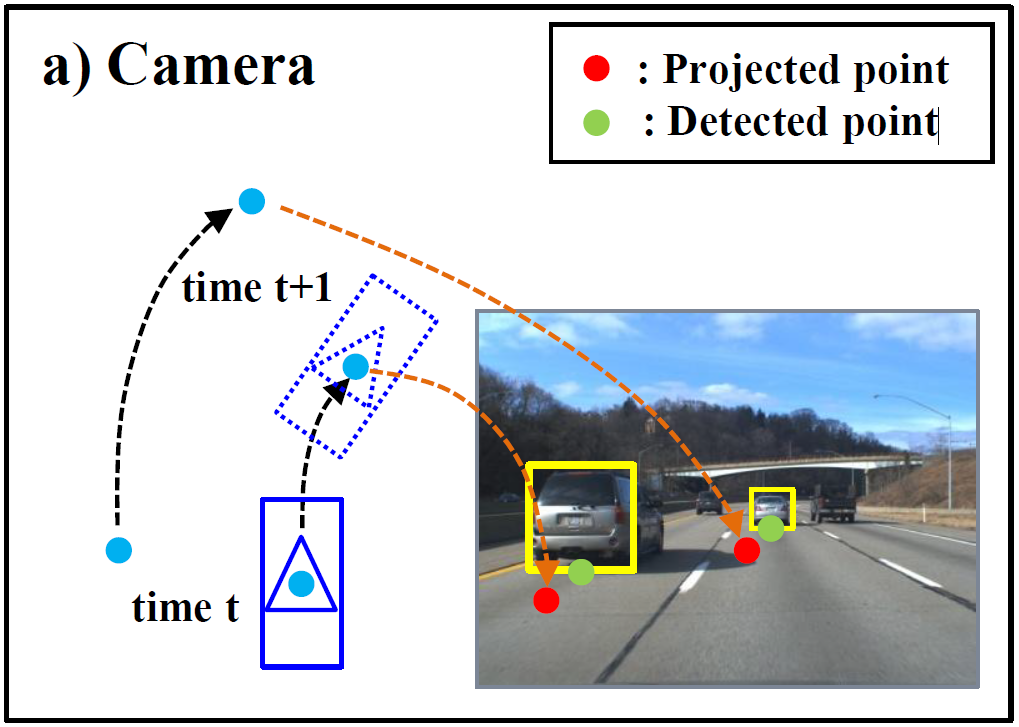
\includegraphics[width=\textwidth]{src/pic/obstacle_a.png}
        \caption{}
        \label{fig:obstacle_a}
    \end{subfigure}
    \begin{subfigure}[b]{0.3\textwidth}
        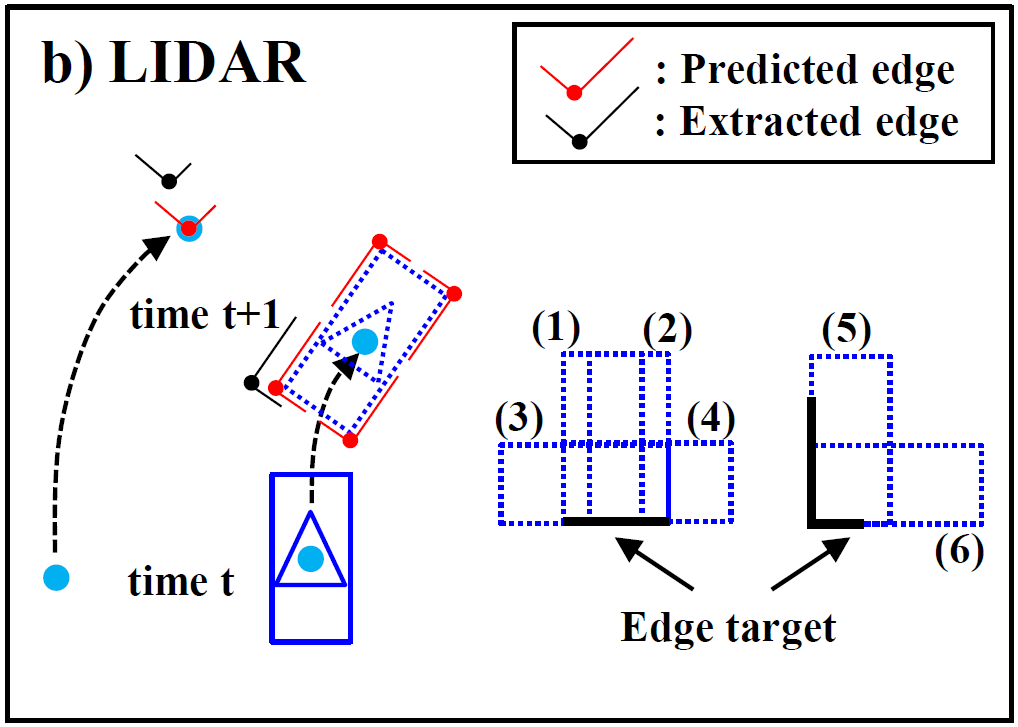
\includegraphics[width=\textwidth]{src/pic/obstacle_b.png}
        \caption{}
        \label{fig:obstacle_b}
    \end{subfigure}
    \begin{subfigure}[b]{0.3\textwidth}
        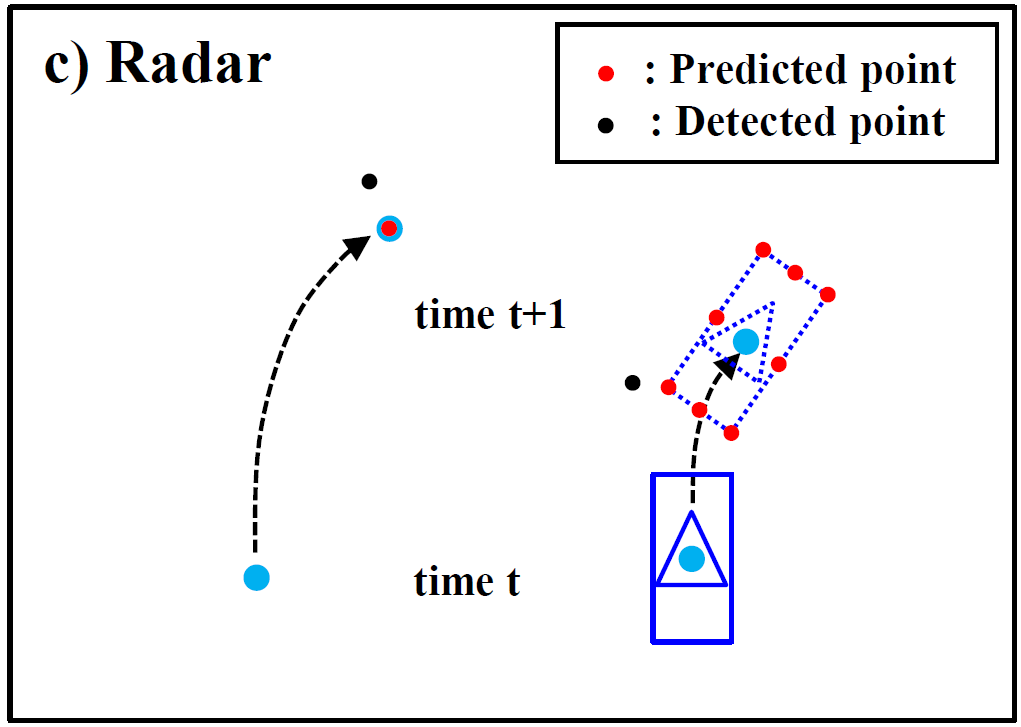
\includegraphics[width=\textwidth]{src/pic/obstacle_c.png}
        \caption{}
        \label{fig:obstacle_c}
    \end{subfigure}
    \caption{\ref{fig:obstacle_a}:, \ref{fig:obstacle_b}:, \ref{fig:obstacle_c}:}
    \label{fig:obstacle}
\end{figure}
\begin{enumerate}[label=\Alph*]
    \item Tracking Models: To demonstrate tracking models, two motion models are chosen as standard i.e., a point model ($M_{P}$), a 3D box model ($M_{B}$). To observe three kinds of sensors three observation models are introduced i.e., Radar($O_{R}$), LIDAR ($O_{L}$) and camera ($O_{C}$) observation model.
    \begin{description}
        \item[Motion Models:] For every moving objects, pedestrians, bicyclists, and cars in this case, the kinematics situations are not same. A pedestrian has the probability to move in any direction in any time. But for the bicyclists or cars, the movement is confined by non-holonomic constraints\cite{Cho_2014}. Motion estimation is performed using point model and 3D box model where it is assumed that a point model moves with a constant acceleration\cite{Cho_2014}. The 3D box model is a bicycle model wit its estimated 3D cuboid\cite{Cho_2014}.
        \item[Observation Models:] In order to capture the point target, the Radar observation model ($O_{R}$) is used. The LIDAR observation model ($O_{L}$) is responsible for modeling a box target. Finally the camera observation model ($O_{C}$) handle the bounding box measurements in the image plane. In practice, the bounding box are not used to update the motion estimation because the depth is uncertain. In \cite{Cho_2014}, the detection results are used to estimate the width and the height of an object and determines objects’ classes. But it can not be used to object initialization or terminate of objects. When the image frames are ready, the length and width is calculated by subtracting the pixel and the 3D height calculated based on camera geometry.
    \end{description}
    \item Data Association: The association of the current state with the previous state is a very critical task. To do the task optimally, some improvements has to be done in the  previous data association algorithm\cite{Cho_2014}.
    
    For camera observations(also called vision targets), the center of determined moving object is projected as either in a point or a box model on the next image frame under the pinhole camera model. After projection, a search is done due to find the nearest point that reduce the distance between the projected point and the middle of the bottom line of the detected bounding boxes. After that the camera observation and its object classification is instantiated. Figure \ref{fig:obstacle_a} shows the details about vision targets.
    
    For LIDAR observations(also called edge targets), a set of possible alignments of edge targets are generated depending on the predicted moving objects. There are four alignment for a box model and one for each point model\cite{Cho_2014}. The extracted targets are associated to the closest predicted one and which reduces the distance between the projected point and the middle of the bottom line of the detected bounding boxes. For utilization, edge targets tracking takes help from vision targets. For example, if the vision target focus on the rear view then it ignores the vehicles side view alignments. Figure \ref{fig:obstacle_b} shows the details about edge targets.
    
    For radar observations(also called point targets), a set of possible point targets is generated from the predicted moving object hypotheses\cite{Cho_2014}. Since radars are usually poor in determining a lateral position of an object, when a tracked object is modeled as a 3D box model, we generate multiple points along the contour of the box model. If an object is tracked through a point model, we generate a single point\cite{Cho_2014}. Figure \ref{fig:obstacle_c} shows the details about point targets.
    
    \item Movement Classification: It is the only goal of tracking is to know if the target is a moving or non-moving object. There are several scenarios of moving object. One object can move continuously, it may move a little bit and stop or stop a little bit then start. To track all of the scenarios, a series of states of a moving objects needs to be keep. In \cite{Cho_2014}, two movement flags are introduced. One is the movement history i.e., observed moving and not observed moving and another on is the movement state, i.e., moving and not moving\cite{Cho_2014}. As radar has build in functionality to track the moving objects, radar is the key component of tracking. Also the motion is compared with a threshold which is statistically determined by testing various vehicles. The movement history classification, the distance traveled is computed from the last time stamp that the object has been classified as not observed moving\cite{Cho_2014}. Here, the distance is also compared with a threshold. Though it is hard to find out the perfect threshold value, it is possible to get an realistic optimal value.
\end{enumerate}


\subsubsection{Experimental Outcome}
The improved version of the tracking system shows a very good performance in real time\cite{Cho_2014}. Some improved cases are described in the following. When a vehicle is tracked in the range of 150m, the tracking system track it as a point model. But when the vehicle comes near at least 40m from the host vehicle the tracking system automatically tracked it as a 3D box model. It is one of the most important feature of self driving car. Because the car should know the exact dimension of the moving object as it come near or go far\cite{Cho_2014}. On the other hand, for pedestrians/bicyclists the range is up to 20m on the experiment vehicle's path.

\section{Sensor-Independent Fusion Approach}
In the area of "Autonomous Driving", it is a very basic idea to use multiple sensors and to fuse the sensors data to determine something which can not be determined by just evaluating the sensors data separately. The sensors are hardware module which are accessed by a very complex software module to handle the sensor data and operate the vehicle. Meanwhile, different sensors module may have different software dependency which makes the changeability of sensor harder. There could be several reasons to change the sensors, but the main two reasons are: 
\begin{enumerate}
    \item Add more sensors to increase reliability or systems Field of View (FOV)\cite{Kunz_2015}
    \item Replacing costly sensors with the cheaper ones, with a reduced for example, to make the system available for cheaper cars. So, if there is a need of replacement or enhancement, the software module is also needs to be updated or redeveloped.
\end{enumerate}
So, if there is a need of replacement or enhancement, the software module is also needs to be updated or integrated with new code. In the paper \cite{Kunz_2015}, a modular multi-sensor sensor independent fusion system is proposed where sensor independent means it can accept any kind of sensor. It would be possible in that system that, changing the sensors does not involved software changes. This sensor independent approach ensures redundancy and replaceable using sensor-independent probabilistic interfaces\cite{Kunz_2015}. From the view point of performance, this system could provide good performance in the occurrence of temporary malfunction or degradation of individual sensors.

\subsection{Environment Setup}
Foe the experiment, a Mercedes-Benz E-Class car is selected and modified to enable autonomous features. The modification includes, A Paravan Space-Drive steering system which enables moving the steering by wire, a modified ESP(electronic stability program) control unit which enables to directly specify the break and acceleration torque\cite{Kunz_2015}. To perform the high level computational tasks, two computers are installed in the trunk and they could perform parallel.

\subsection{Sensors Used}
Three sensors are installed in the experiment vehicle. They are installed in a way that, it is hardly visible from outside and integrated in the body. There are three IBEO LUX laser scanners are set in the front bumper. They have the ability to scan maximum range of up to 200m at front and the angle of 210$^{\circ}$. There is also a front facing monochrome camera is installed behind the windshield with a resolution of 1392 x 1040 px. Moreover, the car is equipped with seral radar sensors. A Frequency Modulated Continuous Wave (FMCW) based Continental ARS 310 automotive long-range radar is mounted underneath the grille\cite{Kunz_2015}. The radars have the range of o.25m to 200m. The sensor coverage is visualized in the fig \ref{fig:sensor_covarage_Independent}. To cover the rear view, a radar is mounted centered behind the rear bumper and two reward facing cameras are mounted hehind the rear window. Besides all of these sensors, A real-time kinematic (RTK) system in combination with a differential GPS is used for mapping and evaluation\cite{Kunz_2015}.
\begin{figure}
  \centering
  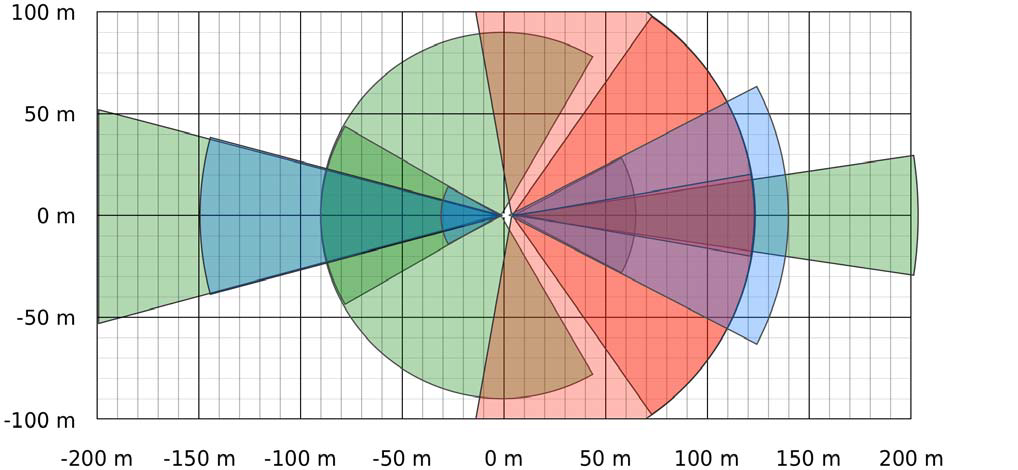
\includegraphics[width=.6\textwidth]{src/pic/sensor_covarage_Independent.png}
  \caption{The front face of the vehicle is in the right direction.  Sensor coverage: cameras(blue), laser scanners (red), radar sensors (green) \cite{Kunz_2015}}
  \label{fig:sensor_covarage_Independent}
\end{figure}
\subsection{Sensor Fusion}
According to \cite{Kunz_2015}, in a multi-sensor system it is highly recommended to utilize all of the sensors data. One sensor may recover the draw backs of other sensors. For example, A radar has build in functionality to give accurately the position and velocity of moving object. But the yaw angle is uncertain. To recover this drawback of radar we could use a mono camera which can not provide velocity information but it can provide an accurate yaw angle.


\subsection{Experimental Outcome}




% \chapter{Code Listings}\label{ch:listings}
%% use language 'myLng' for the next listings (until another language is set)
%% include listing 'listings/AdverseReactionApp.aj' with label and caption
%% note: big listings sometimes need to overwrite the float value that has been
%% already set in the general listings setup (see paper.tex)

This chapter contains the beautiful listing \ref{lst:system}. 
Lorem ipsum dolor sit amet, consetetur sadipscing elitr, sed diam nonumy 
eirmod tempor invidunt ut labore et dolore magna aliquyam erat, sed diam 
voluptua. At vero eos et accusam et justo duo dolores et ea rebum. Stet 
clita kasd gubergren, no sea takimata sanctus est Lorem ipsum dolor sit 
amet. Lorem ipsum dolor sit amet, consetetur sadipscing elitr, sed diam 
nonumy eirmod tempor invidunt ut labore et dolore magna aliquyam erat, 
sed diam voluptua. At vero eos et accusam et justo duo dolores et ea 
rebum. Stet clita kasd gubergren, no sea takimata sanctus est Lorem 
ipsum dolor sit amet. 




\begin{figure}[hbt]
\lstset{language=MontiArc}
\lstinputlisting[
label=lst:system,
caption=Code listing with user defined syntax highlighting (MontiArc).] {src/listings/AdverseReactionApp.aj}
\end{figure}

\cleardoublepage


\chapter{Conclusion}



\bibliographystyle{abbrv}
\addcontentsline{toc}{chapter}{Bibliography}
\bibliography{src/bib/Literatur}

% Begin Anhang
% \appendix
% \chapter{z.\,B. Programmdokumentation}

\cleardoublepage


\end{document}
